\chapter{Architecture}
\label{chap:math}

\section{Model}
\label{sec:model}
There are many models for sentiment analysis of financial news, and each has its advantages and disadvantages. Some of these models are based on traditional statistical methods, while others are based on deep learning.

Among the latest and best models are those based on the Transformer architecture, which are capable of high accuracy and can process large amounts of data. Some of the most well-known ones include BERT (Bidirectional Encoder Representations from Transformers) by Google or GPT (Generative Pre-trained Transformer) by OpenAI.

\subsection{BERT}
\label{sec:bert}
Bidirectional Encoder Representation from Transformer is one of the most popular state of the art text embedding model published by Google. One of the reasons BERT is more successful is that it uses a context based embedding model. Without context, the word would have the same meaning in both sentences. 

BERT looks at the sentence and figures out what words is related to in the sentence, and will create embedding of the word based on the context. BERT does this by using transformers, which is a state of the art deep learning architecture, that is mostly used for Natural language processing. The architecture uses encoder-decoder paradigm.

\subsection{GPT}
\label{sec:gpt}

\section{Data}
\label{sec:data}

\subsection{Train data}
\label{sec:train_data}

Use some datasets from kaggle to train model.

\subsection{Real time data}
\label{sec:real_time_data}

Description of data scraping algorithm and analysis of valid sources.

\section{Example with some mathematics}
\label{sec:demo}

\begin{defn}[Triplet]\label{defn:x}
Given stuff $X$, $Y$ and $Z$, we will write a \emph{triplet} of the stuff as $(X,Y,Z)$.
\end{defn}

\newcommand{\Col}{\textsc{Colour}}

\begin{thm}[Car coloring]\label{thm:y}
All cars have the same color. More specifically, for any set of cars $C$, we have
$$(\forall c_1, c_2 \in C)\:\Col(c_1) = \Col(c_2).$$
\end{thm}

\begin{proof}
Use induction on sets of cars $C$. The statement holds trivially for $|C|\leq1$. For larger $C$, select 2 overlapping subsets of $C$ smaller than $|C|$ (thus same-colored). Overlapping cars need to have the same color as the cars outside the overlap, thus also the whole $C$ is same-colored.\todo{This is plain wrong though.}
\end{proof}

\begin{figure}
\centering
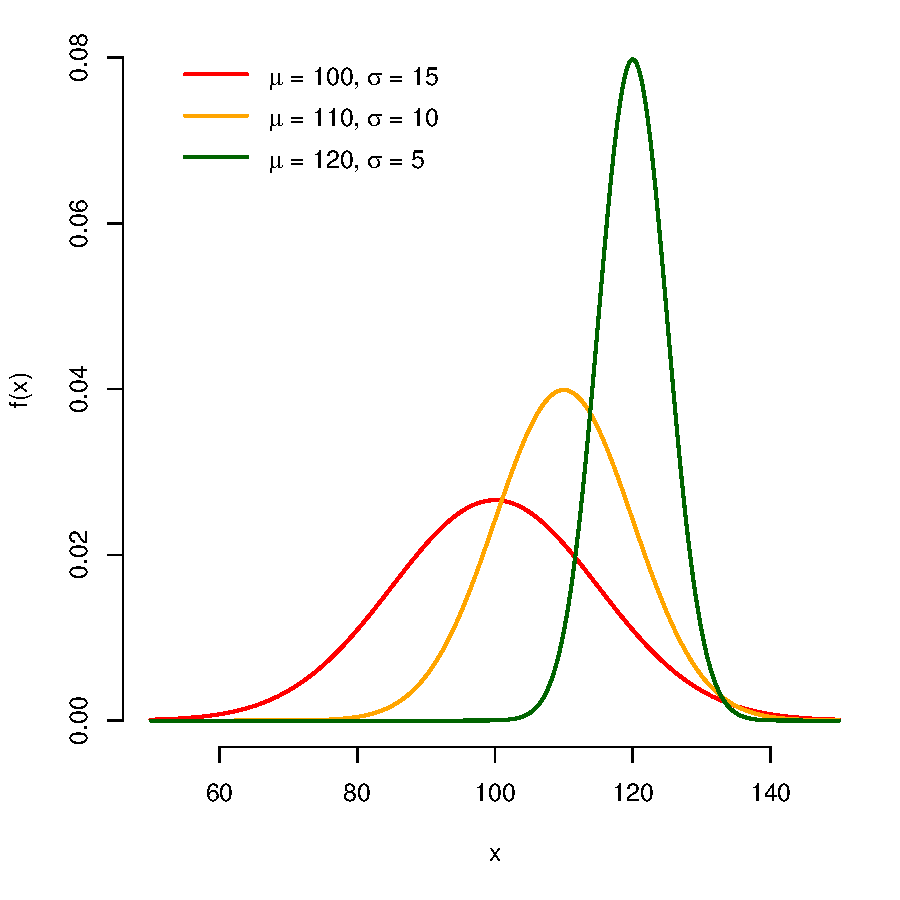
\includegraphics[width=.6\linewidth]{img/ukazka-obr02.pdf}
\caption{A figure with a plot, not entirely related to anything. If you copy the figures from anywhere, always refer to the original author, ideally by citation (if possible). In particular, this picture --- and many others, also a lot of surrounding code --- was taken from the example bachelor thesis of MFF, originally created by Martin Mareš and others.}
\label{fig:g}
\end{figure}

\begin{figure}
\centering
\tikzstyle{box}=[rectangle,draw,rounded corners=0.5ex,fill=green!10]
\begin{tikzpicture}[thick,font=\sf\scriptsize]
\node[box,rotate=45] (a) {A test.};
\node[] (b) at (4,0) {Node with no border!};
\node[circle,draw,dashed,fill=yellow!20, text width=6em, align=center] (c) at (0,4) {Ugly yellow node.\\Is this the Sun?};
\node[box, right=1cm of c] (d) {Math: $X=\sqrt{\frac{y}{z}}$};
\draw[->](a) to (b);
\draw[->](a) to[bend left=30] node[midway,sloped,anchor=north] {flow flows} (c);
\draw[->>>,dotted](b) to[bend right=30] (d);
\draw[ultra thick](c) to (d);

\end{tikzpicture}
\caption{An example diagram typeset with TikZ.}
\label{fig:schema}
\end{figure}

\begin{algorithm}
\begin{algorithmic}
\Function{ExecuteWithHighProbability}{$A$}
	\State $r \gets$ a random number between $0$ and $1$
	\State $\varepsilon \gets 0.0000000000000000000000000000000000000042$
	\If{$r\geq\varepsilon$}
		\State execute $A$ \Comment{We discard the return value}
	\Else
		\State print: \texttt{Not today, sorry.}
	\EndIf
\EndFunction
\end{algorithmic}
\caption{Algorithm that executes an action with high probability. Do not care about formal semantics in the pseudocode --- semicolons, types, correct function call parameters and similar nonsense from `realistic' languages can be safely omitted. Instead make sure that the intuition behind (and perhaps some hints about its correctness or various corner cases) can be seen as easily as possible.}
\label{alg:w}
\end{algorithm}

\section{Extra typesetting hints}

Do not overuse text formatting for highlighting various important parts of your sentences. If an idea cannot be communicated without formatting, the sentence probably needs rewriting anyway. Imagine the thesis being read aloud as a podcast --- the storytellers are generally unable to speak in boldface font.

Most importantly, do \underline{not} overuse bold text, which is designed to literally \textbf{shine from the page} to be the first thing that catches the eye of the reader. More precisely, use bold text only for `navigation' elements that need to be seen and located first, such as headings, list item leads, and figure numbers.

Use underline only in dire necessity, such as in the previous paragraph where it was inevitable to ensure that the reader remembers to never typeset boldface text manually again.

Use \emph{emphasis} to highlight the first occurrences of important terms that the reader should notice. The feeling the emphasis produces is, roughly, ``Oh my --- what a nicely slanted word! Surely I expect it be important for the rest of the thesis!''

Finally, never draw a vertical line, not even in a table or around figures, ever. Vertical lines outside of the figures are ugly.
